\section{Objectif des tests}

	Dans cette partie, nous allons exposer quels tests nous avons effectué ainsi que 
	la méthodologie utilisée.
	Nous avons plusieurs attentes que vous souhaitons évaluer avec des tests. \newline
	 
	Tout d'abord, dans le processus de réalisation de l'algorithme, nous devons nous assurer 
	que notre implémentation est correcte. Nous souhaitons également vérifier par des tests 
	sur du matériel dédié les hypothèses émises plus tôt dans ce travail [ \hyperref[hyp]{\ref{hyp}} ], 
	à savoir : vérifier que les surcoûts augmentent avec le nombre de cœurs, de tâches, 
	de périodes différentes. 
	Nous chercherons à confronter des résultats théoriques avec une réalisation.
	Nous pouvons également comparer la charge des processeurs avec \textbf{Global-EDF} pour des mêmes ensembles de tâches.

%	Nous voulons :
%	\begin{enumerate}
%	\setlength\itemsep{0.1em}
%		\item Montrer qu'on a implémenté le bon algorithme
%		\item Regarder les temps de surcoût sur des tests basiques
%		\begin{enumerate}
%			\item mesurer les WCET
%			\item mesurer les temps d'exécution et retirer tout ce qui n'est pas de l'exécution = overhead
%			\item voir si ça augmente bien avec le nombre de cœur, avec plus ou moins de tâches
%		\end{enumerate}
%		\item voir si avec des tâches de périodes harmoniques, on arrive à des trucs sympas
%		\item mesurer le temps d'occupation des procs
%		\item comparer pour tout ça avec Global-EDF
%		\item trouver des trucs faisables avec UEDF, pas faisables avec global, et inversement
%	\end{enumerate}
	

\section{Matériel utilisé}
	\textbf{HIPPEROS} est peut être installé sur un nombre limité de machines. 
	L'une d'elle est une \textbf{SABRE Lite} dont voici les spécifications :
	
	\subsubsection{SABRE Lite i.MX6}
		\begin{enumerate}
			\setlength\itemsep{0.1em}
			\item Architecture \textbf{ARMv7} \textbf{Cortex-A9}
			\item Processeur Freescale i.MX6 Quad 1GHz
			\item 1 GB de ram
			\item Mémoire sur carte micro-SD
		\end{enumerate}
	C'est un kit de développement couramment utilisé. Les spécifications qui 
	ont vraiment de l'importance ici sont le nombre de cœurs et la mémoire ram, 
	le reste étant assez secondaire dans les tests que nous réalisons.

\section{Création de tâche}

	\subsubsection{Description de tâche dans HIPPEROS}
	Pour exécuter des tâches avec \textbf{HIPPEROS}, il faut définir des fichiers de configuration 
	sous un format \textit{XML}, dans ce fichier doivent apparaître certaines propriétés des tâches. 
	Dans notre cas :
	\begin{itemize}
		\setlength\itemsep{0.1em}
		\item le nom
		\item l'adresse de l'exécutable
		\item Si elles sont en temps réel
		\item Si elles ont une ou plusieurs occurrences \{\textit{OneShot; Periodic; Sporadic}\}
		\item leur WCET
		\item leur période
		\item leur échéance
	\end{itemize}
	et ceci autant de fois que de tâches que l'on aura à décrire. \newline
	
	Les tests que nous faisons passer doivent nous permettre de contrôler au mieux la durée réelle 
	d'exécution de la tâche, afin de maîtriser l'écart entre cette valeur et le WCET attribué dans les 
	fichiers de configuration. \newline
	
	Pour ce faire, nous créons un unique programme qui sera lancé autant de fois que de tâches déclarées 
	dans le fichier de configuration. 
	Nous définissons un fichier de \textit{header} contenant un tableau de valeurs. 
	Ainsi, lors de chaque exécution, le programme va lire une valeur dans un tableau, qui représente la 
	limite de temps qu'il devra atteindre avant de se terminer proprement.\newline
	
	Concrètement, un programme \textbf{Measure} possède un \textit{Process Id}, et exécute cette boucle :

	\label{algomeasure}
	\begin{algorithm}[H]
		\caption{Measure\_main}
		\begin{algorithmic}
			\STATE $boundary \leftarrow BoundaryList[Process\_id] + now$
			\REPEAT \item $t = now$
			\UNTIL{ $t < boundary$ }
		\end{algorithmic}
	\end{algorithm}

	Cette tâche périodique est relancée autant de fois que nécessaire; c'est à dire qu'à la fin 
	d'une boucle, elle est suspendue, puis réactivée à chaque période.
	
	\subsubsection{Déroulement d'un test}
	Nous créons un fichier contenant les informations utiles sur le test :
	\begin{itemize}
		\item WCET
		\item Offset
		\item Période
		\item Échéance
	\end{itemize}
	Nous exécutons ensuite les programmes compilés sur la \textit{SABRE Lite}, en nous assurant qu'il n'y a pas 
	de dépassement de WCET ou de période. Lorsque l'ensemble a été validé en test, il sera 
	exécuté plus longuement (1 à 2h) afin d'être analysé ultérieurement.\newline

	Il est important de signaler ici qu'\textbf{HIPPEROS} permet de générer des \textit{logs}.
	En branchant sur port USB une sonde, il est possible de récupérer 
	un certain nombre d'informations sur port série, comme ces événements :
	\begin{itemize}
		\item la tâche est (ré)activée
		\item le travail démarre son exécution
		\item le travail est préempté
		\item le travail est arrêté
	\end{itemize}
	Il y a un décalage entre le moment des décision et le moment d'exécution de cette décision. Par exemple, il peut s'écouler un temps relativement long 
	entre la décision de dispatcher un travail sur un cœur et le début de l'exécution. Les logs rendent un peu compte de cet écart 
	quoi qu'il faut avoir conscience qu'eux-mêmes faussent les données.
	En effet, la production de logs prend un certain temps en provoquant des écritures 
	sur le port série.
	Par conséquent, les résultats présentés ici ne peuvent 
	être considérés autrement que comme des approximations.\newline
	
	À titre d'illustration, voici l'exemple sur un de nos tests du décalage entre 
	le moment où une certaine tâche est dispatchée et le début de son exécution.

	
\begin{figure}[H]
	\label{4tasksdispatch}
	\caption{Temps écoulé entre une décision et le début d'une exécution}
	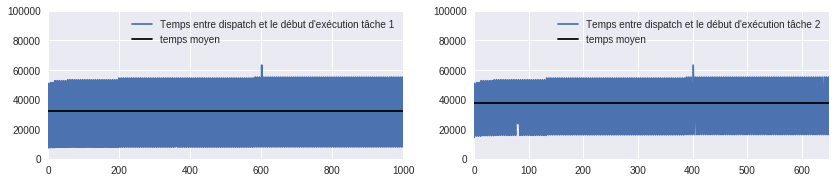
\includegraphics[scale=0.5]{img/wcet/dispacth1}
	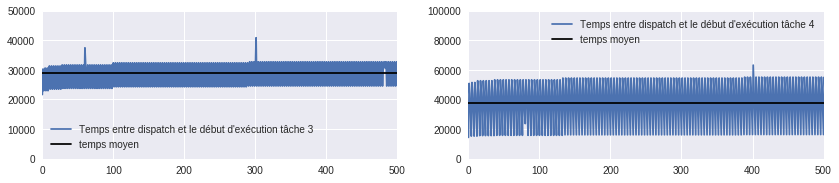
\includegraphics[scale=0.5]{img/wcet/dispacth2}
\end{figure}
	
	
	
\section{Génération des ensembles}

Nous ne disposons pas d'un générateur aléatoire de tâches, et ce pour les raisons que nous allons exposer maintenant.
L'ordonnanceur \textbf{UEDF} est fort sensible aux valeurs des périodes et WCET, puisque 
c'est avec l'\textit{utilisation} qu'il réserve du temps d'exécution sur chaque cœur. 
Concrètement, on imagine bien qu'en générant de façon aléatoire des WCET, ces proportions sur les 
périodes ne donneront pas forcément une valeur entière.\newline

Imaginons un cas de figure où la somme des utilisations des $n$ tâches de priorités supérieures 
n'atteint la somme de $101\%$, dans ce cas, une tâche va réserver $1\%$ de son WCET 
sur un cœur avant de devoir être préemptée, puis migrée sur le cœur précédent. Ce comportement 
serait trop contraignant et nous risquons de ne pas avoir de résultats intéressant à 
proposer. De plus, l'industrie procède généralement à une génération de tâches de périodes harmoniques, 
si bien que ce choix se défend également de ce point de vue.
Néanmoins, cela pourrait faire partie d'un travail ultérieur.\newline

Pour créer un ensemble de tâches, nous générons un nombre aléatoire de périodes différentes, 
ainsi qu'un multiple de la première période. Nous ne sommes donc pas 
avec une classe de tâches de périodes harmoniques uniquement, 
mais proches de ce cas de figure.\newline

Nous précisons également que les tests que nous avons faits passer comportent 
un nombre peu élevé de tâches, allant de $6$ à $12$, la majorité étant des 
ensembles de $10$ tâches. C'est un ordre de grandeur qui s'approche d'un cas d'utilisation industriel, 
qui nous permettait d'obtenir des résultats avec des propriétés différentes, et conserve 
l'utilité des résultats obtenus.


\section{Détermination des WCET des tâches}\label{methodo}
	\textbf{UEDF} est optimal, en \underline{théorie}. Revenons un instant sur ce point. 
	Cela signifie que si aucun ordonnancement pour un système donné existe, 
	aucun autre ordonnanceur ne pourra l'ordonnancer.\newline

	%\todo{ajouter blabla sur scope du WCET et que c'est documenté + liens trouvés}	
	En pratique, le WCET d'une tâche est une valeur difficile à donner, et qui va dépendre de 
	beaucoup de facteurs.\newline
	
	Elle dépend :
	\begin{enumerate}
		\item du nombre d'opérations à faire dans le code (approximation du nombre d'instructions) et de leur type (IO, calcul...)
		\item de la plateforme d'exécution de la tâche (les caractéristiques de la machine)
		\item de l'algorithme d'ordonnancement, des surcoûts.
	\end{enumerate}
	
	\subsection{Nombre et type d'opération}
	Le pire temps d'exécution peut varier en fonction du nombre d'instructions et surtout de leur type. En effet, 
	on peut penser qu'une tâche qui doit uniquement faire du calcul prend un temps déterministe, en pratique, 
	il y aura toujours quelques modifications. \newline
	Par ailleurs, certaines instructions prennent un temps plus ou moins variable. Par exemple, 
	les entrées-sorties ont un temps qui peut fort varier. En outre, selon la disponibilité ou 
	des ressources, des temps peuvent s'ajouter. 
	
	\subsection{La plateforme d'exécution}
	Pour des raisons évidentes, une tâche ne mettra pas un temps équivalent sur une plateforme ou sur une autre, 
	et le temps n'est donc pas une propriété théorique de la tâche elle-même mais dépend bien 
	également de la plateforme. On peut bien avoir une idée en comptant le nombre d'instructions et en faisant 
	des calculs par rapport à la fréquence du processeur, mais cela reste approximatif. 
	Cela peut néanmoins suffire dans le cas de systèmes non-critiques.\newline
	
	Dans un cas idéal où le WCET ne dépendrait que de la machine et du nombre d'instructions, 
	on aurait pu imaginer faire un certain nombre d'exécutions de la même tâche et prendre une valeur 
	statistiquement en dehors des valeurs possibles avec certitude de $n\%$. %\todo{nommer ce test statistique}

	\subsection{L'ordonnanceur}
	
	En fin de compte, l'ordonnanceur va ici avoir un impact sur le WCET. 
	Concernant \textbf{Global-EDF}, le WCET ne fait pas partie des paramètres utilisés pour calculer 
	l'ordonnancement. La variable déterminante est l'échéance absolue ($d_i(t)$). 
	Le WCET en revanche est déterminant dans le cas d'\textbf{UEDF}. Voyons 
	l'impact de cette variable et les risques liés à l'évaluation de cette valeur.\newline
	
	En bref rappel de la partie \hyperref[contexte]{Contexte [ \ref{contexte} ]}, 
	Le WCET va permettre de calculer l'\textit{utilisation} de la tâche. 
	Cette proportion est utilisée pour déterminer le nombre d'unités de temps d'exécution 
	du travail $i$ attribuées au processeur $\pi_j$. \newline
	Nous savons qu'il y a un temps plus ou moins long entre la décision d'exécuter et le moment 
	où le travail débute son exécution. Ceci explique pourquoi au moment de commencer les tests, 
	il est très difficile d'évaluer le rapport entre les temps d'exécutions 
	moyens des tâches et les WCET que nous devons fixer. \newline
	
	Cette procédure d'évaluation a consisté au départ à paramétrer très manuellement les WCET et 
	durées d'exécutions demandées, pour proposer finalement une façon plus systématique 
	de fixer ces valeurs.


\section{Rapport WCET vs temps d'exécution moyen}

La première difficulté rencontrée lors de la mise en place de tests a été de déterminer la façon 
de configurer les ensembles afin que ceux-ci soit ordonnançables sans provoquer de 
dépassement de WCET ou d'échéances tout en conservant une charge de travail la plus élevée possible, et ce, dans le 
but de mesurer l'évolution des surcoûts.

D'après nos tests, la façon de déterminer les WCET par rapport à la durée moyenne d'exécution de la tâche 
dépend du type d'ensemble, 
du nombre de tâches ainsi que du nombre de cœurs utilisés (donc de la somme des \textit{utilisations} de l'ensemble).
Nous pouvons en revanche considérer qu'en fixant comme WCET environ le double 
de la durée moyenne d'exécution, nous laissons une marge suffisante. En effet, nous avons commencé 
par mesurer l'évolution d'une de nos tâches sur un cœur afin de voir si sa durée d'exécution était 
stable ou non.

\begin{figure}[H]
	\label{evotask}
	\caption{Évolution du temps d'exécution moyen d'une tâche}
	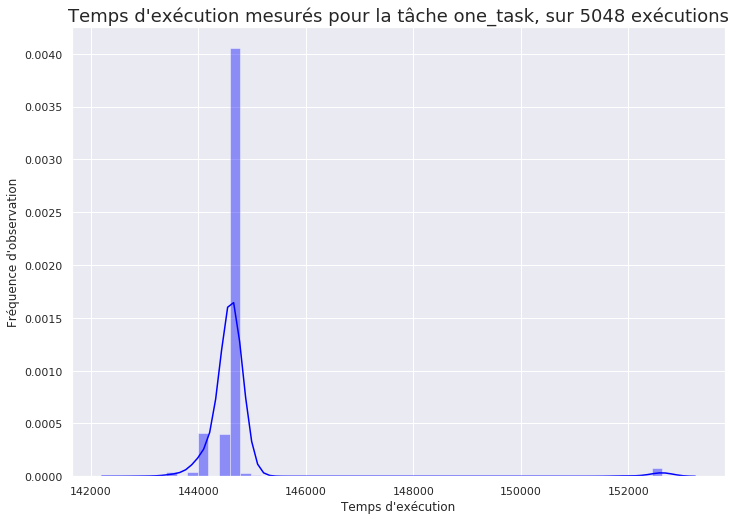
\includegraphics[scale=0.5]{img/wcet/one_task_hist}
\end{figure}

Ce graphique nous montre qu'une variabilité existe bien, mais les extremums restent très proche de la valeur moyenne.

Nous avons finalement opté pour donner des valeurs de WCET d'environ deux fois plus grandes que les durées 
d'exécution moyennes, ceci étant basé sur nos nombreux essais. 

	
\section{Récolte des résultats}
	Afin de pouvoir analyser les performances de l'implémentation d'\textbf{UEDF}, il nous faut être capable de reconstituer 
	l'historique d'une exécution. \newline
	
	Cela est possible en produisant des sorties (\textit{logs}) que nous parsons à l'aide d'outils 
	développés en \textit{Python}. 
	

\section{Comparaison avec G-EDF}

	Les expériences réalisées avec \textbf{UEDF }ont toutes été également réalisées avec \textbf{Global EDF}.
	Les mêmes ensembles de tâches ont été rejoués en changeant juste l'ordonnanceur. 
	
	
\section{Premiers tests de calibration, somme d'utilisation de 100 \%}

Pour une somme des utilisations de $100\%$, \textbf{UEDF} va se comporter comme un ordonnanceur 
monocore, même s'il dispose de plusieurs cœurs. Cela ne présente pas beaucoup d'intérêt d'étudier la 
répartition de la charge, puisque ce résultat est totalement attendu.\newline

En revanche, la configuration -- autrement dit : le calibrage -- diffère, puisque 
\textbf{Global-EDF} n'utilise pas du tout le WCET pour prendre ses décisions, contrairement 
à \textbf{UEDF}. Cette donnée doit donc être fixée avec une grande attention.\newline

Ce premier graphique montre l'évolution de la charge du cœur $0$ dans une série d'ensembles dont la 
somme des utilisations ($\sum_0^{n-1}U(i)$) est de $100\%$.
Cela nous permet de tester plus facilement l'évolution de la charge possible d'un processeur en fonction du nombre de tâches.\newline

Un ensemble est choisi s'il ne provoque pas de dépassement de WCET ou d'échéance durant une exécution 
mais qu'en variant de quelques dizaines de millisecondes la durée moyenne d'exécution de la tâche, une de ces erreurs arrive. 
Cela signifie que l'on s'approche par essai/erreur de la limite au delà de laquelle nous trouvons un dépassement.\newline

Les premières courbes montrent l'évolution du rapport entre les temps d'exécution moyens et les WCET renseignés dans la 
configuration de la tâche. 
Dans ce premier test, nous avons exécuté et analysé l'exécution de $5$ ensembles de tâches composés respectivement de 
$2$, $3$, $4$, $6$ et $8$ tâches.\newline 

Par construction, la première courbe indique l'évolution pour des tâches de périodes toutes égales comme référence, 
et la seconde indique l'évolution sur base de périodes de soit harmoniques, soit proches de l'harmonie.\newline


\begin{figure}[H]
	\label{evowcethomogene}
	\caption{Évolution de la charge d'utilisation en fonction du nombre de tâches, somme d'utilisation de 100$\%$}
	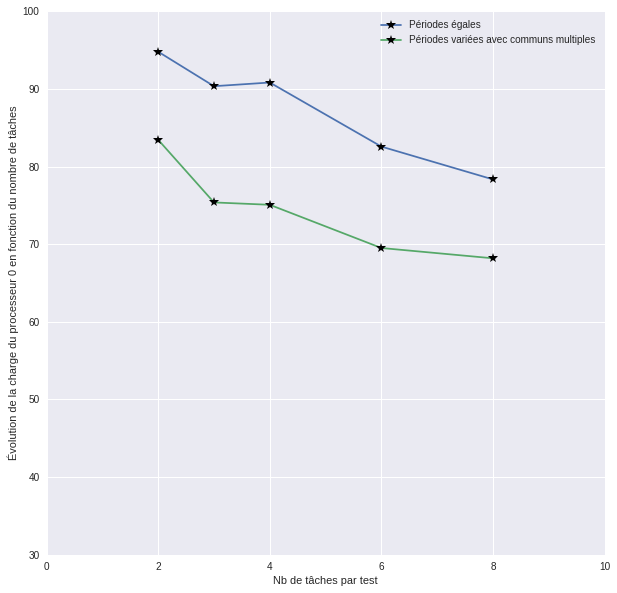
\includegraphics[scale=0.6]{img/wcet/load_100u}
\end{figure}

Cette illustration est ainsi développée dans ce travail afin de montrer l'effort de calibration, ainsi que 
de démontrer une différence avec d'autres ordonnanceurs pour lesquels le calcul du WCET des tâches est 
sans doute moins crucial. À l'issue de cette analyse, ainsi que d'autres essais non détaillés dans ce 
document, nous constatons que le cœur $0$, qui se trouve être le cœur \textit{Master} dans le système d'exploitation \textbf{HIPPEROS}, 
sera fort sollicité à exécuter les décisions, migrations, etc. Une façon simple d'améliorer la répartition de la 
charge sera exposée dans le chapitre \hyperref[perspectives]{Perspectives} [\ref{perspectives}]. 
Sans cette amélioration dans le code, nous forcerons les ensembles ultérieurs 
à avoir une charge bien moins élevée sur le cœur $0$ que sur les autres, ce qui rend les systèmes 
plus facilement ordonnançables. En ayant conscience de la façon de procéder de cet ordonnanceur, 
concrètement, nous seront plus pessimiste sur le temps moyen d'exécution des tâches 
dont les périodes sont les plus petites dans nos tests.